%-------------------------------------------------------------------------------
\section{Code execution procedure}\label{sec:running}
%-------------------------------------------------------------------------------
This section describes how to use the SKYCORR software.
Section~\ref{sec:paramfile} provides an example for an input parameter file.
The input parameters are discussed in detail in Section~\ref{sec:params}.
Finally, the output of the code is described in Section~\ref{sec:output}. In
Section~\ref{sec:calling} the execution of the programme is shown. For the
extraction of 1D spectra suitable for SKYCORR from 2D FITS images, see
Section~\ref{sec:extract1d}. The run of examples is described in
Section~\ref{sec:calling_examples}. The SKYCORR software also provides a Reflex
workflow. It is discussed in Section~\ref{sec:reflex}.

%-------------------------------------------------------------------------------
\subsection{Input parameter file}\label{sec:paramfile}
%-------------------------------------------------------------------------------
All parameters needed for the fit are read from an ASCII parameter file, which
contains parameter names, descriptions, and initial values. In the following,
{\tt src/test/config/sctest\_sinfo\_H.par} is shown as an example of a
parameter file. Individual parameters are explained in
Section~\ref{sec:params}:

{\small
\begin{verbatim}
# ----------------------------------------------------------------------------
# -------------------- INPUT PARAMETER FILE FOR SKYCORR ----------------------
# ----------------------------------------------------------------------------

# ---------------------------DIRECTORIES + FILES------------------------------

# Absolute path of skycorr installation directory
INST_DIR=../../

# Absolute or relative (with respect to INST_DIR) path and filename of input
# object spectrum
INPUT_OBJECT_SPECTRUM=src/test/data/sky_sinfo_1.fits

# Absolute or relative (with respect to INST_DIR) path and filename of input
# sky spectrum
INPUT_SKY_SPECTRUM=src/test/data/sky_sinfo_2.fits

# Absolute or relative (with respect to INST_DIR) path and filename of output
# directory (will be created if not present; default: <INST_DIR>/output/)
OUTPUT_DIR=output

# Main name of diagnostic output files, extensions will be added
OUTPUT_NAME=TEST-SINFO-H

#------------------------------INPUT STRUCTURE--------------------------------

# Names of file columns (table) or extensions (image)
# A list of 4 labels has to be provided:
# 1: wavelength [image: NONE if dedicated extension does not exist]
# 2: flux [image: NONE if in zeroth, unnamed extension]
# 3: flux error [NONE if not present]
# 4: mask (integer: 1 = selected, 0 = rejected;
#          float:   0. = selected, otherwise rejected) [NONE if not present]
COL_NAMES=lambda flux NONE NONE

# Error relative to mean if no error column is provided (default: 0.01)
DEFAULT_ERROR=0.01

# Multiplicative factor to convert wavelength to micron
# e.g.: wavelength unit = A -> WLG_TO_MICRON = 1e-4
WLG_TO_MICRON=1.

# Wavelengths in vacuum (= vac) or air (= air)
VAC_AIR=vac


# ----------------------------------------------------------------------------
# ------------------------- EXPERT MODE PARAMETERS ---------------------------
# ----------------------------------------------------------------------------

# ------------------------------FITS KEYWORDS---------------------------------

# FITS keyword of sky spectrum for Modified Julian Day (MJD) or date in years
# (default: MJD-OBS; optional parameter for value: DATE_VAL)
DATE_KEY=MJD-OBS

# FITS keyword of sky spectrum for UTC time in s
# (default: TM-START; optional parameter for value: TIME_VAL)
TIME_KEY=TM-START

# FITS keyword of sky spectrum for telescope altitude angle in deg
# (default: ESO TEL ALT; optional parameter for value: TELALT_VAL)
TELALT_KEY=ESO TEL ALT

# ---------------------------REQUIRED INPUT DATA------------------------------

# Airglow line list
# Required directory: <INST_DIR>/sysdata/
LINETABNAME=airglow_groups.dat

# File for airglow scaling parameters
# Required directory: <INST_DIR>/sysdata/
VARDATNAME=airglow_var.dat

# FTP address (supplemented by "ftp://") for folder with monthly averages of
# solar radio flux at 10.7 cm
SOLDATURL=ftp.geolab.nrcan.gc.ca/data/solar_flux/monthly_averages

# File with monthly averages of solar radio flux at 10.7 cm
# Required directory: SOLDATURL or <INST_DIR>/sysdata/
SOLDATNAME=solflux_monthly_average.txt

# Solar radio flux at 10.7 cm:
# Positive value in sfu (= 0.01 MJy) or -1 [default] for corresponding monthly
# average from http://www.spaceweather.gc.ca. Download only if local file in
# <INST_DIR>/sysdata/ does not contain required month.
SOLFLUX=-1

# ---------------------------LINE IDENTIFICATION------------------------------

# Initial estimate of line FWHM [pixel]
FWHM=5.0

# Variable line width (linear increase with wavelength)? -- 1 = yes; 0 = no
VARFWHM=0

# Relative FWHM convergence criterion (default: 1e-2)
LTOL=1e-2

# Minimum distance to neighbouring lines for classification as isolated line:
# <MIN_LINE_DIST> * <FWHM> [pixel]
MIN_LINE_DIST=2.5

# Minimum line peak flux for consideration of lines from airglow line list:
# <FLUXLIM> * <median flux of identified lines>
# Automatic search -> FLUXLIM = -1 (default)
FLUXLIM=-1

# ---------------------------FITTING OF SKY LINES-----------------------------

# Relative chi^2 MPFIT convergence criterion (default: 1e-3)
FTOL=1e-3

# Relative parameter MPFIT convergence criterion (default: 1e-3)
XTOL=1e-3

# Relative chi^2 convergence criterion for iterative improvement of
# wavelength grid (default: 1e-3)
WTOL=1e-3

# Maximum degree of Chebyshev polynomial for wavelength grid correction:
# -1 = no correction
#  0 = linear term (coef. = 1) is also considered but not fitted
#  7 = default
CHEBY_MAX=7

# Minimum degree of Chebyshev polynomial for wavelength grid correction.
# CHEBY_MIN <= CHEBY_MAX:
# - Iterative increase of polynomial degree at least until CHEBY_MIN
#   (default: 3).
# - Procedure stops if chi^2 gets worse or CHEBY_MAX is reached.
# - Results of degree with best chi^2 are taken.
# CHEBY_MIN > CHEBY_MAX:
# - Iterative increase of polynomial degree until CHEBY_MAX is reached.
# - Results of degree CHEBY_MAX are taken.
CHEBY_MIN=3

# Initial constant term for wavelength grid correction (shift relative to half
# wavelength range)
CHEBY_CONST=0.

# Type of rebinning:
# 0 = simple rebinning (summation of pixel fractions)
# 1 = convolution with asymmetric, damped sinc kernel [default]
REBINTYPE=1

# Minimum relative weight of the strongest line group of a pixel for
# including a pixel in the line fitting procedure (default: 0.67)
WEIGHTLIM=0.67

# Sigma limit for excluding outliers (e.g. object emission lines) from
# estimate of group flux correction factors (default: 15.)
SIGLIM=15.

# Lower relative uncertainty limit for the consideration of a line group for
# the fitting procedure. The value is compared to the sigma-to-mean ratio of
# the group-specific flux correction factors of the initial estimate
# (default: 0. -> include all fittable line groups).
FITLIM=0.

# ---------------------------------PLOTTING-----------------------------------

# Diagnostic gnuplot plots:
# Options for output on screen:
# W - wxt terminal
# X - x11 terminal
# N - no screen output [default]
# NOTE: An illustration of the sky subtraction quality is plotted into a PS
#       file in the OUTPUT_DIR folder in any case.
PLOT_TYPE=N
\end{verbatim}
}

%-------------------------------------------------------------------------------
\subsection{Parameter description}\label{sec:params}
%-------------------------------------------------------------------------------
In the following, the individual parameters are explained in more detail in the
order as they appear in the parameter file. The file is divided into two parts.
The first part contains the parameters which provide the paths, file names, and
data structures. They have to be adapted if the input and output data files
change. However, the sky correction code can be run without modifying the
parameters of the second part, which affect the sky correction optimisation.
The modification of these so-called expert mode parameters can improve the sky
subtraction provided that the user is willing to run the code several times in
order to find the optimal parameter set.

{\bf\large\tt Basic parameters:}
\begin{itemize}
\item {\sc inst\_dir}: Installation directory for the data reduction task. In
the case of automatic installation (see Section\,\ref{sec:installscript}), this
has to be an absolute path and must be the same as given during the
installation procedure.
\item {\sc input\_object\_spectrum}: Absolute or relative (with respect to
{\sc inst\_dir}) path and name of the input object spectrum for the sky
subtraction procedure. Currently, \ac{ASCII} tables, \ac{FITS} tables with one
table extension, and 1D \ac{FITS} images are allowed. The number of table
columns or \ac{FITS} file image extensions is not restricted. However, only
a single column/extension with flux data can be provided. Corresponding
columns/extensions for flux errors and mask values are also possible. See also
{\sc col\_names}.
\item {\sc input\_sky\_spectrum}: Absolute or relative (with respect to
{\sc inst\_dir}) path and name of the reference input sky spectrum for the sky
subtraction procedure. For the accepted file formats, see
{\sc input\_object\_spectrum}.
\item {\sc output\_dir}: Absolute or relative (with respect to {\sc inst\_dir})
path to the output directory. The folder will be created if it does not exist.
\item {\sc output\_name}: Unique name space for output files. The extensions
{\it \_sci.fits}, {\it \_sky.fits}, {\it \_fit.fits}, {\it \_fit.ps}, and
{\it .res} are added. See Section~\ref{sec:output} for more details.
\item {\sc col\_names}: Column names of the two input files containing
information on wavelength, flux, flux error, and mask. The latter two are
optional and can be disabled by setting them to {\it NONE}. An example
would be the following string: {\it lambda flux NONE NONE}. {\it Blanks} are
used as column name separators. For \ac{ASCII} files, which have to provide the
columns in the given order, the column names are irrelevant, with the exception
of {\it NONE} input. In the case of \ac{FITS} images, the given labels are
compared to the \ac{FITS} extension names (keyword ``EXTNAME''). If there is no
extension name for the spectral flux, it is expected to be present in the first
layer of the \ac{FITS} file (0th extension). In this case, the flux column name
has to be set to {\it NONE}. The name of the wavelength column should also be
{\it NONE}, if the wavelength grid is derived from \ac{FITS} header keywords.
This is the typical situation for \ac{FITS} images. By default, it is expected
that an optional mask has only the values 0 and 1 for rejection and selection,
respectively. Alternatively, pixels with a mask value of 0 are selected
(reverse definition) if the other values (to be rejected) do not equal 1 and
are floating-point numbers.
\item {\sc default\_error}: Default error relative to the mean in the case of
a lacking error column (column name = {\it NONE}, see previous record).
\item {\sc wlg\_to\_micron}: Multiplicative factor to convert input wavelength
unit to micron. For example, for nm this parameter has to set to $10^{-3}$.
\item {\sc vac\_air}: Wavelengths of the input spectra in vacuum ({\it vac}) or
air ({\it air}).
\end{itemize}

{\bf\large\tt Expert mode parameters:}
\begin{itemize}
\item {\sc date\_key}: \ac{FITS} keyword of {\sc input\_sky\_spectrum} for
Modified Julian Day (MJD) or date in years. By default, {\it MJD-OBS} is taken.
If \ac{ASCII} files are provided or no suitable \ac{FITS} keyword is available,
the information has to be provided manually (see below).
\item {\sc date\_val}: MJD or date in years for {\sc input\_sky\_spectrum}.
This parameter is only required if a suitable \ac{FITS} header is not provided
by the input spectrum.
\item {\sc time\_key}: \ac{FITS} keyword of {\sc input\_sky\_spectrum} for UTC
time in seconds. By default, {\it TM-START} is taken. If {\it TM-START} is not
available, an equivalent keyword could be {\it UTC}. If \ac{ASCII} files are
provided or no suitable \ac{FITS} keyword is available, the information has to
be provided manually (see below).
\item {\sc time\_val}: UTC time in seconds for {\sc input\_sky\_spectrum}. This
parameter is only required if a suitable \ac{FITS} header is not provided by
the input spectrum.
\item {\sc telalt\_key}: \ac{FITS} keyword of {\sc input\_sky\_spectrum} for
telescope altitude angle in deg. By default, {\it ESO TEL ALT} is taken. If
\ac{ASCII} files are provided or no suitable \ac{FITS} keyword is available,
the information has to be provided manually (see below).
\item {\sc telalt\_val}: Telescope altitude angle in deg for
{\sc input\_sky\_spectrum}. This parameter is only required if a suitable
\ac{FITS} header is not provided by the input spectrum.
\item {\sc linetabname}: Name of the input airglow line list. The file must be
located in the directory {\tt <inst\_dir>/ sysdata}.
\item {\sc vardatname}: File for the scaling parameters of the airglow
variability model described in Section~\ref{sec:airglow}. The file must be
located in the directory {\tt <inst\_dir>/ sysdata}.
\item {\sc soldaturl}: FTP address (supplemented by {\it ftp://}) for folder
with monthly averages of the solar radio flux at 10.7\,cm. Currently, the link
is provided by {\tt www.spaceweather.gc.ca} and can be obtained via ftp by
\url{ftp.geolab.nrcan.gc.ca/data/solar_flux/monthly_averages}.
\item {\sc soldatname}: Name of file with monthly averages of the solar radio
flux at 10.7\,cm. The file must be located in the directory
{\tt <inst\_dir>/sysdata}. The radio flux is taken from the column
{\it obsflux}. If the data for the required month (as derived from the
\ac{FITS} header) is not present in the local file, the latter is substituted
by the most recent file of the same name in the remote {\sc soldaturl} folder.
In the case of errors a solar radio flux of 130\,sfu is assumed, which
corresponds to the mean of the solar cycles 19 to 23.
\item {\sc solflux}: Solar radio flux at 10.7\,cm in sfu~(= 0.01 MJy). The
default value of -1 results in using the corresponding monthly average from the
file {\sc soldatname}.
\item {\sc fwhm}: Initial guess for the FWHM of the airglow lines in pixels.
This start value is improved by an iterative approach (see
Section~\ref{sec:FWHM}). The width of the sky lines is required for line
identification as well as for the computation of the airglow model.
\item {\sc varfwhm}: Flag for selecting a constant (= 0) or a variable line
width (= 1). In the latter case, all FWHM values are related to the central
wavelength of the full wavelength range. The variable FWHM increases linearly
with wavelength, \ie\ the resolution is constant. X-Shooter Echelle spectra
show this behaviour. For spectra where the object profile in the slit mainly
determines the FWHM, the default constant width option is recommended.
\item {\sc ltol}: Relative FWHM convergence criterion for iterative derivation
of the mean line width in the object and reference sky spectrum (see
Section~\ref{sec:FWHM}). The default is $1 \times 10^{-2}$. In the case of 1,
the code would just use the first FWHM estimate without further iteration.
\item {\sc min\_line\_dist}: Minimum distance to neighbouring lines divided by
the FWHM. This factor is required for the line finding algorithm.
\item {\sc fluxlim}: Minimum line peak flux for including lines from the
airglow line list {\sc linetabname} in the fit. The given value is multiplied
by the median flux of the lines directly identified in the spectrum (see
Section~\ref{sec:linesearch}). The default value of -1 indicates an iterative
approach for the selection of line list entries that aims at including as
many lines as possible without loosing too many pixels for the continuum
interpolation (see Sections~\ref{sec:linesearch} and ~\ref{sec:contsub}). If
the warnings ``no isolated lines found'' and ``all weights =~0'' should appear,
it might help to select a {\sc fluxlim} value below the start value 0.005 of
the automatic search.
\item {\sc ftol}: Relative $\chi^2$ convergence criterion of the MPFIT
least-squares minimisation algorithm for the adaptation of the reference sky
spectrum to the sky in the object spectrum (see Section~\ref{sec:linefit}).
The default is $1 \times 10^{-3}$, \ie, if $\chi^2$ changes between two
iterations by less than 0.1\% the fitting process is stopped.
\item {\sc xtol}: Relative parameter convergence criterion. {\sc xtol} has a
similar functionality as {\sc ftol} but for the fit parameter values instead of
$\chi^2$. The default is $1 \times 10^{-3}$.
\item {\sc wtol}: Relative $\chi^2$ convergence criterion for iterative
adaptation of the wavelength grid of the reference sky spectrum to the grid of
the object spectrum (see Section~\ref{sec:wavegrid}). The degree of the
Chebyshev polynomial that is used to correct the wavelength solution is
increased by 1 for each new iteration. If the resulting $\chi^2$ does not
show a relative improvement of {\sc wtol} and more, the convergence is reached
and the procedure is stopped if {\sc cheby\_min} is not larger than the
polynomial degree of the ongoing iteration (see below). The default is
$1 \times 10^{-3}$.
\item {\sc cheby\_max}: Maximum degree of Chebyshev polynomial for refined
wavelength solution (see Section~\ref{sec:wavegrid}). The special case -1
indicates that no adaptation of the wavelength grid is performed. If a degree
of 0 is chosen, the linear term is always applied and taken into account with
a coefficient of 1. This value is fixed during the fit and cannot be omitted.
The default value is 7.
\item {\sc cheby\_min}: Minimum degree of Chebyshev polynomial for refined
wavelength solution (see Section~\ref{sec:wavegrid}). The iterative increase
of the polynomial degree in the course of the fitting procedure is performed
at least until {\sc cheby\_min} is reached. By default, the minimum degree is
3. If the procedure stops directly after the iteration with a degree of
{\sc cheby\_min}, the results of the iteration with the best $\chi^2$ are
taken. Choosing a {\sc cheby\_min} value higher than {\sc cheby\_max} (\eg\ 99)
results in keeping the results for {\sc cheby\_max}, regardless of the fitting
results for lower polynomials with potentially better $\chi^2$.
\item {\sc cheby\_const}: Constant term of the Chebyshev polynomial for the
wavelength solution. The given value represents a shift relative to half the
wavelength range of the input spectrum. By default, 0 is assumed. Since the
linear term and the higher terms are set to 1 and 0, respectively, at the
beginning, the fitting procedure starts without a wavelength correction if the
default setting is used.
\item {\sc rebintype}: Flag specifying the rebinning algorithm for adapting
the modified sky spectrum to the input sky spectrum (see
Section~\ref{sec:wavegrid}). There are two options. For a value of 0 the
rebinning is based on a summation of pixel fractions. A value of 1 selects the
more sophisticated default rebinning method, which is based on a convolution
with a pixel-dependent, asymmetric, damped sinc kernel. The latter method is
particularly useful for input spectra with significant ($> 0.1$\,pixels)
differences in the wavelength grids.
\item {\sc weightlim}: Minimum relative weight of the strongest line group of
a pixel for including a pixel in the line fitting procedure (see
Section~\ref{sec:linefit}). The relative threshold can be set to values in the
range $0 - 1$. In the former extreme case all spectrum pixels and in the latter
case pixels with only a single line group are included in the line flux and
wavelength correction procedure. The default value is 0.67, \ie, a pixel is
considered if the dominating group is at least twice as strong as the second
group. Since the group weights are crude estimates based on the time-dependent
airglow model discussed in Section~\ref{sec:airglow}, the selected cut tends to
be diffuse for realistic group weights.
\item {\sc siglim}: $\sigma$-limit for excluding outliers (\eg\ object emission
lines) from the sky line fitting procedure. The standard deviation $\sigma$ is
derived from the ratio of the object and sky line peaks. The default value is
15.
\item {\sc fitlim}: Lower relative limit for the consideration of a line group
for the fitting procedure. The initial estimate of the line group scaling
factors results in a mean and an RMS scatter for each group. Then, groups
are included for fitting if the $\sigma$-to-mean ratio is above the provided
parameter value. By default {\sc fitlim} is 0, which selects all groups with at
least one valid line for the fitting procedure. A high value of \eg\ 100 would
avoid the use of MPFIT for the line strength correction. Simple line group
scaling would be applied only, which is very fast but tends to be less accurate
than the fitting procedure.
\item {\sc plot\_type}: Optional output of diagnostic plots on the screen using
either a wxt (W) or an x11 (X) terminal. The default N indicates that no screen
output is produced. Independent of the choice of this parameter a postscript
plot with a comparison between the input object spectrum and the best-fit sky
spectrum is written to {\sc output\_dir} (see Section~\ref{sec:output}).
\end{itemize}

%-------------------------------------------------------------------------------
\subsection{Output files}\label{sec:output}
%-------------------------------------------------------------------------------
%-------------------------------------------------------------------------------
\subsubsection{Output overview}
%-------------------------------------------------------------------------------
The output files produced by the sky correction code are stored in the
directory specified by the {\sc output\_dir} parameter. The following output
files (named corresponding to the {\sc output\_name} parameter) are created:
\begin{itemize}
\item <{\sc output\_name}>\_sci.fits: input science spectrum converted into
a \ac{FITS} table. Columns names are taken from {\sc col\_names}. In the case
of {\it NONE} for wavelength and flux, {\it LAMBDA} and {\it FLUX} are taken.
Independent of the presence of a mask column in the original data, an integer
mask column with 0 for rejection and 1 for selection is added. If a mask column
name is available, {\it \_I} is suffixed. Otherwise it is called {\it MASK\_I}.
\item <{\sc output\_name}>\_sky.fits: input sky spectrum converted into a
\ac{FITS} table. For details on the column names, see above.
\item <{\sc output\_name}>\_fit.fits: full \ac{FITS} table of the sky
correction procedure for diagnostic purposes with the following columns:
  \begin{itemize}
  \item {\it lambda}: wavelength of input science spectrum in micron
  \item {\it flux}: flux of input science spectrum
  \item {\it dflux}: flux error of input science spectrum (only present if
        available)
  \item {\it mask}: integer mask of input science spectrum (only present if
        available)
  \item {\it weight}: reciprocal of error or 0 for masked pixels in the input
        science spectrum
  \item {\it class}: flag for line identification (0 = continuum pixel,
        1 = line pixel, 2 = line peak, 3 = isolated line peak for FWHM
        estimation)
  \item {\it cflux}: continuum flux of science spectrum
  \item {\it lflux}: line flux of science spectrum
  \item {\it mcflux}: rebinned continuum flux of reference sky spectrum
  \item {\it mlflux}: rebinned line flux of modified reference sky spectrum
  \item {\it mflux}: adapted reference sky spectrum (sum of {\it mcflux} and
        {\it mlflux})
  \item {\it mdflux}: flux error in adapted reference sky spectrum (only
        present if available)
  \item {\it mmask}: rebinned integer mask of reference sky spectrum (only
        present if available)
  \item {\it mweight}: rebinned weight of reference sky spectrum
  \item {\it sigclip}: $\sigma$-clipping of pixels depending on ratio of
        science and sky line flux (0 = no clipping, 1 = clipped)
  \item {\it cweight}: resulting pixel weight combining {\it weight},
        {\it mweight}, and {\it sigclip}
  \item {\it dev}: weighted difference between {\it mlflux} and {\it lflux}
        (for $\chi^2$ calculation)
  \item {\it scflux}: sky-subtracted science spectrum (difference between
        {\it flux} and {\it mflux})
  \item {\it scdflux}: flux error in sky-subtracted science spectrum (only
        present if available)
  \item {\it scmask}: integer mask of sky-subtracted science spectrum (only
        present if available)
  \end{itemize}
\item <{\sc output\_name}>\_fit.ps: postscript plot showing a comparison of the
best-optimised reference sky spectrum, the input science spectrum, and the
difference of both spectra.
\item <{\sc output\_name}>.res: results file containing information on the
quality of the sky correction procedure and the best-fit parameters (see
Section~\ref{sec:resfile}).
\end{itemize}

Apart from the intermediate and diagnostic products, a file with the sky
subtraction results is written in {\sc output\_dir} that has the same file
format as the input science spectrum. The original file name is complemented by
``\_SC''. In the case of \ac{ASCII} and \ac{FITS} tables, the columns
{\it scflux}, {\it scdflux}, and {\it scmask} are added to the input data. The
latter two columns are only present if flux error and mask columns are already
provided by the input file. In the case of a \ac{FITS} image, the data in the
flux extension is substituted by the sky-subtracted flux. Similar operations
are performed for optional flux error and mask extensions. If a non-integer
mask is provided by the input file, the integer mask values from {\it scmask}
are converted (see also {\sc col\_names} in Section~\ref{sec:params}). In the
case of \ac{FITS} files, an extended header with keywords related to the sky
correction procedure is written into the first \ac{FITS} layer.

%-------------------------------------------------------------------------------
\subsubsection{Example of a {\tt .res} file}\label{sec:resfile}
%-------------------------------------------------------------------------------
The <{\sc output\_name}>.res contains detailed information on the fit results.
In particular, information on the fit quality, \ie\ $\chi^2$ and r.m.s values,
the line FWHM estimation, all coefficients of the best-fit model, and their
uncertainties are given. For a description of the provided status message, see
the documentation in {\tt mpfit.h}. In general, positive numbers imply that the
code found a solution. In the case of status 99, no fitting could be performed
due to a lack of suitable lines. In this special case, the reference sky
spectrum is simply subtracted from the object spectrum.

In the following, the output file belonging to the parameter file listed in
Section~\ref{sec:paramfile} is shown:
\begin{verbatim}
INPUT DATA FILES:
Science: evaluation/data/sky_sinfo_1.fits
Sky:     evaluation/data/sky_sinfo_2.fits

MPFIT RESULTS:
Status:                 1
Fit parameters:         27
Data points:            1921
Weight > 0:             510
MPFIT calls:            9
Iterations:             37
Function evaluations:   587
Fit run time in s:      8.08
Initial chi2:           5.229e+04
Best chi2:              3.744e+04
Reduced chi2:           7.768e+01
RMS rel. to error:      8.814e+00
Full RMS:               3.150e+03
Full RMS rel. to peaks: 1.918e-02
Line RMS rel. to peaks: 2.314e-02
Peak RMS rel. to peaks: 2.991e-02
Mean rel. residual:     2.853e-02

ESTIMATED SPECTRAL RESOLUTION:
FWHM in pixels: 3.325

BEST-FIT PARAMETERS:

Type N  Fit     Value                RMS        N_lin
A    30  0       2.333 +- 9.99       9.99       0
A    31  1       2.965 +- 0.0188     0.1124     11
A    32  1       2.528 +- 0.01604    0.03491    23
A    33  1       2.268 +- 0.0144     0.04689    34
A    34  1       1.992 +- 0.01263    0.05744    31
A    35  1        1.84 +- 0.01168    0.05968    22
A    36  0       2.333 +- 9.99       9.99       0
A    47  1       4.494 +- 0.2091     0.8258     18
B    01  1       1.233 +- 0.00794    0.01799    4
B    02  1       1.242 +- 0.007881   0.01401    15
B    03  1       1.217 +- 0.007788   0.01507    8
B    04  1       1.238 +- 0.007854   0.01515    19
B    05  1        1.25 +- 0.007979   0.06325    10
B    06  1       1.248 +- 0.007944   0.02035    16
B    07  1       1.268 +- 0.00823    0.04584    11
B    08  1       1.198 +- 0.007695   0.02138    13
B    09  1       1.118 +- 0.008475   0.02639    5
B    10  1       1.153 +- 0.007893   0.09762    8
B    21  1       1.772 +- 0.0837     0.3374     3
B    22  1       2.077 +- 0.08977    0.08087    2
B    23  1       1.358 +- 0.06366    0.149      4
B    24  1       2.357 +- 0.1192     0.1241     1
w    00  1  -4.717e-06 +- 3.498e-07  9.99       0
w    01  1           1 +- 1.277e-06  9.99       0
w    02  1   1.017e-05 +- 5.767e-07  9.99       0
w    03  1   8.649e-06 +- 3.823e-07  9.99       0
w    04  1           0 +- 4.689e-07  9.99       0

REMARKS:
Type: A/B = line group A/B, w = wavelength fit coef.
Fit: 1 = free MPFIT par., 0 = only initial estimate
RMS: uncertainty of initial estimate
9.99: no error available
N_lin: number of lines for fitting
\end{verbatim}

%-------------------------------------------------------------------------------
\subsection{Executing SKYCORR}\label{sec:calling}
%-------------------------------------------------------------------------------
After the installation, the folder {\tt <INST\_DIR>/bin/} contains the
executable. It is invoked by
\begin{verbatim}
    cd <INST_DIR>/
    bin/skycorr <parameter file>
\end{verbatim}
where {\tt <parameter file>} represents a user-defined parameter file
(including paths).

%-------------------------------------------------------------------------------
\subsection{Executing {\tt extract1d}}\label{sec:extract1d}
%-------------------------------------------------------------------------------
After the installation, the folder {\tt <INST\_DIR>/bin/} also contains
a programme for the extraction of 1D spectra for SKYCORR from 2D \ac{FITS}
images. The executable {\tt extract1d} was added especially for X-Shooter
pipeline spectra, which belong to the set of example data (see
Section~\ref{sec:calling_examples}).

Since the current X-Shooter pipeline does not produce 1D sky spectra, they have
to be extracted from 2D spectra. In order to make sure that the number of
extracted sky pixels per wavelelength bin is the same for the sky and the
science spectrum, the extraction of both 1D frames is performed together. For
the extraction, just a fixed pixel range in spatial direction is considered,
which is derived by means of the spatial object profile. Only pixels that have
at least a minimum flux relative to the full flux range indicated by the
profile are selected. By default, this limit is 0.01. It can be changed by
modifying the fourth parameter of {\tt extract1d} (see below). If the input
\ac{FITS} files provide an extension with mask or quality values, this is used
to avoid bad pixels in the extracted 1D science spectrum. The relative
contribution of skipped pixels to the profile function is taken to correct for
changes in the extracted 1D science spectrum due to pixel masking. The
extraction algorithm for the 1D science spectrum is not as elaborate as the
approach used by the X-Shooter pipeline. However, for demonstrating the
performance of SKYCORR, it is required to extract science and sky spectra in a
consistent way. The 1D sky spectrum is derived from the median flux in spatial
direction and then scaled to the effective number of pixels that were used for
the extraction of the 1D science spectrum. For a bright and/or extended object,
the choice of a median, \ie\ taking the pixel at the relative position 0.5 in
flux-sorted pixel list, could be not optimal. For this case, the selected
relative position in the sorted pixel list can be modified by the fifth input
parameter (see below). The values 0.4 or 0.45 could be reasonable for a bright
object.

The executable {\tt extract1d} is invoked by
\begin{verbatim}
    cd <INST_DIR>/
    bin/extract1d <parameter file>
                  <2D FITS image for science spectrum>
                  <2D FITS image for sky spectrum>
                  <minimum relative profile flux>
                  <selected relative position in flux-sorted pixel list>
\end{verbatim}
where {\tt <parameter file>} represents a user-defined parameter file
(including paths). The two input files must have the same file formats and
the instrumental set-up should have been the same. It is possible to use the
same FITS file for the science and sky spectrum. In this case, the performance
of SKYCORR and the extraction algorithm can be compared with the one of the
X-Shooter pipeline (see Section~\ref{sec:calling_examples}).

%-------------------------------------------------------------------------------
\subsection{Executing the sky correction examples}\label{sec:calling_examples}
%-------------------------------------------------------------------------------
After an automatic installation, a series of example input files is located in
the folder \\{\tt <INST\_DIR>/examples/config/}.
The corresponding spectra can be found in the subfolder \\
{\tt <INST\_DIR>/examples/data/}. There are two types of examples in the
{\tt examples/config/} folder.
The names of the parameter files of the first type start with {\tt sctest}.
They comprise examples of spectra from the SINFONI, X-Shooter,
and FORS instruments. These examples are a subset of the spectra studied in
Section~\ref{sec:evaluation}. After automatic installation, they can directly
be tested by invoking
\begin{verbatim}
    bin/skycorr examples/config/<config_file>
\end{verbatim}
in the {\tt <INST\_DIR>/} folder. Note that --in case of a manual
installation of the software-- the paths in the example configuration files
have to be edited accordingly in advance.

The parameter files whose names start with {\tt XPL} represent test data from
the X-Shooter pipeline (V2.0.0; see Modigliani et al. \cite{MOD10}) without sky
subtraction. Before SKYCORR can be run, the provided 2D \ac{FITS} images have
to be converted into 1D \ac{FITS} images. For this purpose, the programme
{\tt extract1d} can be used (see Section~\ref{sec:extract1d}). The required
command-line parameters are provided by the SKYCORR parameter files as comment
lines at the beginning. For convenience, the SKYCORR input files produced by
{\tt extract1d} can already be found in {\tt examples/config/}. The examples
are for all three X-Shooter arms UVB, VIS, and NIR. Set-ups are provided that
use the same 2D spectrum for the 1D science and sky spectrum ({\tt d0h}). On
the other hand, one can also test the situation when the sky spectrum was taken
two hours after the science spectrum ({\tt d2h}). Especially in the case of the
{\tt d0h} files, the results can be compared to the sky-subtracted 1D spectra
from the pipeline. The corresponding reference files are indicated by {\tt ref}
in the file name. A detailed discussion of the X-Shooter examples can be found
in the report \cite{SM03SR}.

%-------------------------------------------------------------------------------
\subsection{Reflex workflow}\label{sec:reflex}
%-------------------------------------------------------------------------------
The SKYCORR package comes along with a workflow embedded in the
Reflex\footnote{\tt https://www.eso.org/sci/software/reflex/} environment. This
workflow provides a graphical user interface to provide the parameter settings
to the underlying SKYCORR base code, and incorporates a plotting routine. For a
detailed description on the usage of Reflex, we refer the reader to the Reflex
User Manual \cite{reflex}. For demonstration purposes, the Reflex workflow is
ready to be run with an example after invoking.

The Reflex workflow canvas contains four sections:
\begin{itemize}
    \item {\bf Input / output paramters}: In this section all required
information on the input / output has to be given. In particular, the directory
structure, file names, and the properties of the input spectra must be provided
here. Note: Do {\it not} change the installation directory. We also highly
recommend not to change the parameters which are marked in light blue. A
comprehensive description of the parameters are given in
Sections~\ref{sec:paramfile} and \ref{sec:params}.
    \item {\bf Fitting parameters:} In this section the fitting parameters can
be modified. A comprehensive description of the parameters are given in
Sections~\ref{sec:paramfile} and \ref{sec:params}. Note: The parameters are not
fully checked for the compatibility with respect to SKYCORR at this stage. If
something goes wrong, a Reflex-based error window occurs and shows -- apart
from the Java messages arising from the underlying Reflex workflow -- also the
SKYCORR error message.
    \item {\bf Workflow instructions:} Here, a short description of the
workflow is given.
    \item {\bf Workflow}: Actual Reflex workflow.
\end{itemize}

After providing all parameters, the workflow can be started by pressing the
`Run' button in the Reflex top menu (see Figure~\ref{fig:buttons}(a)). Now, the
SKYCORR base code is invoked with a parameter file created on basis of the
user-defined parameter set. The usual console output of SKYCORR is suppressed
by Reflex, except in case of an error. To watch the progress, we recommend to
activate the animation provided by Reflex via its main menu (`Tools'
$\rightarrow$ `Animate at Runtime' $\rightarrow$ set value to 1).

After the fit is finished, a plotting window is opened to enable the user to
check the results (see Figure~\ref{fig:sc_gui}). This window provides a toolbar
in the lower left corner, which enables the user to zoom into details (see
Figure~\ref{fig:buttons}(b). By exiting the plot windows (`Exit' button) the
Reflex workflow is finished and can be invoked again. In this way, a best fit
can be achieved iteratively.
\begin{figure}
\centering
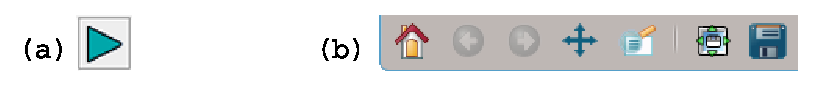
\includegraphics[width=10cm,clip=true,angle=0]{figures/refl_buttons.eps}
\caption[]{(a) `Run' button to start the Reflex workflow; (b) zoom toolbar
provided by the Python library {\tt matplotlib}. With the leftmost symbol, the
user always comes back to the overview; the second and the third symbol enables
the user to go `Back' and  `Forward' in the zooming history; the 4$^{\rm th}$
button shifts the plot via the mouse; the 5$^{\rm th}$ button is the actual
zooming button, which can be used via the mouse; the 6$^{\rm th}$ button opens a
window to configure the subplots; the 7$^{\rm th}$ button saves the plot to a
file.}
\label{fig:buttons}
\end{figure}

\begin{figure}
\centering
\includegraphics[width=21cm,clip=true,angle=-90]{figures/skycorr_reflex.png}
\caption[]{Canvas of the SKYCORR Reflex workflow.}
\label{fig:sc_reflex}
\end{figure}

\begin{figure}
\centering
\includegraphics[width=17cm,clip=true,angle=-90]{figures/skycorr_gui.png}
\caption[]{Plot of the SKYCORR Reflex workflow.}
\label{fig:sc_gui}
\end{figure}

